%%%%%%%%%%%%%%%%%%%%%%%%%%%%%%%%%%%%%%%%%
% Journal Article
% LaTeX Template
% Version 2.0 (February 7, 2023)
%
% This template originates from:
% https://www.LaTeXTemplates.com
%
% Author:
% Vel (vel@latextemplates.com)
%
% License:
% CC BY-NC-SA 4.0 (https://creativecommons.org/licenses/by-nc-sa/4.0/)
%
% NOTE: The bibliography needs to be compiled using the biber engine.
%
%%%%%%%%%%%%%%%%%%%%%%%%%%%%%%%%%%%%%%%%%

%----------------------------------------------------------------------------------------
%	PACKAGES AND OTHER DOCUMENT CONFIGURATIONS
%----------------------------------------------------------------------------------------

\documentclass[
	a4paper, % Paper size, use either a4paper or letterpaper
	10pt, % Default font size, can also use 11pt or 12pt, although this is not recommended
	% unnumberedsections, % Comment to enable section numbering
	twoside, % Two side traditional mode where headers and footers change between odd and even pages, comment this option to make them fixed
]{LTJournalArticle}

\usepackage{
	amsmath,
	tikz,
}

\usetikzlibrary{shapes.geometric, shapes.symbols, arrows, positioning, calc, fit, backgrounds}
\tikzstyle{startstop}=[
    rectangle,
    rounded corners=0.45cm,
    minimum height=0.9cm,
    text centered,
    text width=1.75cm,
    inner sep=0.2cm,
    draw=black,
    fill=black!75,
    text=white,
]

\tikzstyle{document}=[
    tape,
    tape bend top=none,
    text centered,
    text width=1.75cm,
    inner sep=0.2cm,
    draw=black,
]

\tikzstyle{data}=[
    trapezium, 
    trapezium left angle=70, 
    trapezium right angle=110, 
    text width=1.75cm, 
    inner sep=0.2cm,
    text centered, 
    draw=black,
]

\tikzset{
    component top center/.style 2 args={
        rectangle,
        rounded corners=3pt,
        inner sep=0.3cm,
        draw=#2,
        label={[anchor=center, yshift=0.35cm, text=#2]north:#1},
        fill=#2!5
    }
}
\tikzset{
    component bottom center/.style 2 args={
        rectangle,
        rounded corners=3pt,
        inner sep=0.3cm,
        draw=#2,
        label={[anchor=center, yshift=-0.35cm, text=#2]south:#1},
        fill=#2!5
    }
}
\tikzset{
    component bottom left/.style 2 args={
        rectangle,
        rounded corners=3pt,
        inner sep=0.3cm,
        draw=#2,
        label={[anchor=west, yshift=-0.35cm, text=#2]south west:#1},
        fill=#2!5
    }
}

\tikzstyle{block}=[
    rectangle,
    text centered,
    text width=1.75cm,
    inner sep=0.2cm,
    draw=black,
    fill=white,
]

\tikzstyle{summing}=[
    circle,
    draw=black,
    fill=white,
    minimum size=0.5cm,
    path picture={
        \draw [black]
            (path picture bounding box.135) -- (path picture bounding box.315)
            (path picture bounding box.45) -- (path picture bounding box.225);
    }
]

\tikzstyle{arrow}=[
    thick,->,>=stealth,
    text centered,
    inner sep=0.1cm,
]

\tikzstyle{arrow text}=[
    align=center,
    inner sep=0.1cm,
]

\tikzstyle{arrow bridge}=[
    fill=white,
    minimum size=0.33cm,
    path picture={
        \draw[black, thick] (-0.165cm, 0) to (-0.135cm + 0.75pt, 0);                 % left horizontal joint
        \draw[black, thick] (0.165cm, 0) to (0.135cm - 0.75pt, 0);                   % right horizontal joint
        \draw[black, thick] (0, -0.165cm) to (0, 0.025cm);                           % vertical line
        \draw[black, thick] (0.135cm - 0.5pt, -0.25pt) arc (0:180:0.135cm - 0.5pt);  % bridge
    }
]

\DeclareMathOperator*{\argmin}{\arg\!\min}
\DeclareMathOperator*{\argmax}{\arg\!\max}

\addbibresource{bibliography.bib} % BibLaTeX bibliography file

\runninghead{Piranha Plants as Charade} % A shortened article title to appear in the running head, leave this command empty for no running head

% \footertext{\textit{Journal of Biological Sampling} (2024) 12:533-684} % Text to appear in the footer, leave this command empty for no footer text

\setcounter{page}{1} % The page number of the first page, set this to a higher number if the article is to be part of an issue or larger work

%----------------------------------------------------------------------------------------
%	TITLE SECTION
%----------------------------------------------------------------------------------------

\title{Piranha Plants as Charade: Exploring \\ Melody-Guided, Algorithmic Music Generation} % Article title, use manual lines breaks (\\) to beautify the layout

% Authors are listed in a comma-separated list with superscript numbers indicating affiliations
% \thanks{} is used for any text that should be placed in a footnote on the first page, such as the corresponding author's email, journal acceptance dates, a copyright/license notice, keywords, etc
\author{Max Huang$^*$, Emily Yu$^*$}
% \author{%
% 	John Smith\textsuperscript{1,2}, Robert Smith\textsuperscript{3} and Jane Smith\textsuperscript{1}\thanks{Corresponding author: \href{mailto:jane@smith.com}{jane@smith.com}\\ \textbf{Received:} October 20, 2023, \textbf{Published:} December 14, 2023}
% }

% Affiliations are output in the \date{} command
\date{April 4, 2025}
% \date{\footnotesize\textsuperscript{\textbf{1}}School of Chemistry, The University of Michigan\\ \textsuperscript{\textbf{2}}Physics Department, The University of Wisconsin\\ \textsuperscript{\textbf{3}}Biological Sciences Department, The University of Minnesota}

\renewcommand{\maketitlehookd}{%
	\begin{abstract}
		\noindent
        The premise of ``Piranha Plants as Charade'' is to transform a melody into a full-fledged song in the style of ``Piranha Plants on Parade'' from the video game ``Super Mario Bros. Wonder''. Given an input melody in the form of a digital signal (e.g. a WAV file), we developed a music generation algorithm that transforms the input with the following process: 1) it extracts the melodic information from the input; 2) it generates a chord progression that fits under both the extracted melody and the appropriate stylistic conventions; 3) it generates a musical accompaniment based on the melody and chord progression; and 4) it exports the generated accompaniment as a WAV file. For inputs within the targeted scope (i.e. in 4/4, in C major, and at 110 BPM), our algorithm can often produce convincing results, but for a majority of the cases, the output is subpar. Step 1 (melody extraction) is most likely the largest source of failure; the pitch detection is generally correct, however, the onset detection often produces false positives. Despite the current shortcomings, we believe that the core ideas behind ``Piranha Plants as Charade'' can be extended upon to adequately meet the premise we set. We plan on fine-tuning our algorithm and further iterating over our code to produce better results.
	\end{abstract}
}

%----------------------------------------------------------------------------------------

\begin{document}

\maketitle % Output the title section

\def\thefootnote{*}\footnotetext{Equal contribution}\def\thefootnote{\arabic{footnote}}

%----------------------------------------------------------------------------------------
%	ARTICLE CONTENTS
%----------------------------------------------------------------------------------------

\section{Introduction}

\subsection{Motivation}

The fields of mathematics and music are heavily intertwined. In the late 16th-century, many Western European music theorists believed that they had developed \emph{ars perfecta}: a set of rules for which, if followed, guaranteed that music be ``free of reprehensible elements, purged of every error and polished, and [the] harmonies will be good and pleasant'' \autocite{Richard:2005}. Although the concept of perfect music is a footnote in the modern musical landscape, we are intrigued by their aspirations to model musical correctness with rule-based approaches. We wanted to similarly explore the relationship between music and mathematics by generating music using rule-based algorithms that humans follow --- processes that mirror the human composer. Our goal was to create a proof-of-concept computer program that transforms a melody into a full-fledged song in the style of ``Piranha Plants on Parade''\footnote{\href{https://www.youtube.com/watch?v=3EkzTUPoWMU}{youtube.com/watch?v=3EkzTUPoWMU}} from the video game \emph{Super Mario Bros. Wonder}.

\subsubsection{Why ``Piranha Plants on parade''?}

We believe that this was the ideal song to emulate for our proof-of-concept. It is based on a relatively simple harmonic framework, which lets us focus on developing the algorithm's high-level concepts rather than on hard-coding harmonic rules; yet the transitions between harmonic states are distinct enough to be recognizable. Similarly, the song's accompaniment style is repetitive enough such that it can be approximated with only a few rules. ``Piranha Plants on Parade'' also distinctively features gibberish lyrics, which lets us explore vocal generation without worrying about conforming to an existing language. Lastly, the song originates from a video game, a medium with a long history of using synthetic audio and music, thus we believe it to be a thematically appropriate subject for computer-generated music.

\subsection{Minimum Viable Product (MVP)}

We worked on Piranha Plants as Charade for one-and-a-half months --- from February 10 to March 24, 2025 --- and we borrowed ideas from several areas of computer science and music, including but not limited to: digital signal processing (DSP), hidden Markov models (HMM), Western music theory, and Jazz performance. Due to time and budget limitations and our lack of expertise across our explored domains, we believed that it was unreasonable for us to perfectly emulate the style of ``Piranha Plants on Parade''. Thus, our goal was to create an MVP, which we defined as follows:
\begin{enumerate}
    \item The MVP should support melody inputs with the following properties:
    \begin{enumerate}
        \item Has a time signature of 4/4.
        \item Is in the key of C major.
        \item Has a tempo of 110 beats per minute.
        \item Starts on a note (i.e. not a rest).
    \end{enumerate}
    \item For any supported input, the MVP should output a song with the following parts:
    \begin{enumerate}
        \item The input melody and a harmony line, both sung in a `Piranha Plant style'.
        \item A stride piano part that outlines an appropriate chordal accompaniment.
    \end{enumerate}
\end{enumerate}
We consider Piranha Plants as Charade to have adequately met our MVP goals. We also implemented additional features, including exported percussion parts and live deployment in the form of an application programming interface (API).

\section{System Overview}

Given an input melody in the form of a digital signal, we developed a music generation algorithm that transforms the input with these steps: 1) extract the melodic information from the input; 2) generate a chord progression that fits under both the extracted melody and the appropriate stylistic conventions; 3) generate a musical accompaniment based on the melody and chord progression; and 4) export the generated accompaniment as a WAV file (see Figure \ref{fig:architecture}).

\subsection{Melody Extraction}
\label{sec:melody_extraction}

The first step in Piranha Plants as Charade is to extract the melody from the input audio. The goal of this section is to take an audio file and output a sequence of notes, each with a MIDI pitch, start time, and duration. This problem can be broken down into two subproblems: pitch detection and note segmentation.

As a pre-processing step, we first apply the Harmonic-Percussive Source Separation (HPSS) algorithm \autocite{HPSS:2010,HPSS:2014} to separate the harmonic and percussive components of the audio signal. We perform pitch detection on the harmonic component and use the percussive component to identify the timestamps where notes start, which we refer to as note onsets. Finally, we combine both components to produce the final sequence of notes.

\subsubsection{Pitch Detection}

This problem determines the fundamental frequency of a sound; we aim to produce a sequence of MIDI pitches that correspond to notes in the melody. We explored a few different approaches, starting with cepstrum analysis and autocorrelation. However, these methods failed to handle the complexity of audio sourced from non-ideal environments. We elaborate more upon this in Section \ref{sec:avenues}. We decided to use the PYIN algorithm as implemented in the librosa library, which is a state-of-the-art pitch detection algorithm that builds upon autocorrelation to detect pitches more robustly.

The PYIN algorithm \autocite{PYIN:2014} is robust on imperfect audio and has a readily available implementation in the librosa library\footnote{\href{https://librosa.org/doc/0.11.0/generated/librosa.pyin.html}{librosa.org/doc/0.11.0/generated/librosa.pyin.html}}, which allowed us to focus on the higher-level aspects of our project. PYIN is a state-of-the-art pitch detection algorithm that builds upon autocorrelation to handle audio more robustly. At a high level, PYIN applies autocorrelation to detect pitch candidates and refines the result using a probabilistic thresholding model to filter out spurious frequencies.

After applying PYIN to the harmonic component of the audio signal, we have the estimated pitch in hertz across time. We then apply multiple pitch shifts by a few cents \footnote{A logarithmic unit representing a hundredth of a semitone.} to find the best match, determined by the lowest error after rounding to the nearest MIDI pitch.

\subsubsection{Note Segmentation}

Once we have the pitch sequence, it must be segmented into individual notes. To do this, we count quantized time units from the start of the first identified pitch at the assumed tempo of the song. Within each interval, we take the mode of the pitches as the pitch at that time. We end the previous note and begin a new one if either of the following conditions are met:
\begin{enumerate}
    \item The pitch changes from the previous interval.
    \item An onset is detected in the percussive component of the audio at the corresponding time.
\end{enumerate}
Thus, we obtain a sequence of notes defining the melody to pass to the next component.


\subsection{Chord Generation}

[chord generation]


\subsection{Accompaniment Generation}
\label{sec:accompaniment_generation}

Like many human composers, our accompaniment generation process follows a rule-based approach. With the melody and chord progression from Parts \ref{sec:melody_extraction} and \ref{sec:chord_generation} as context, it generates different parts for each instrument using algorithms conceptualized from a music theory point of view. This is similar to how a Jazz musician, who is familiar with the conventions of the genre, can use lead sheets\footnote{A minimalist type of music notation that contains the melody and chord changes in a song.} as context to determine what to play in an ensemble. Unlike in this analogy, the different parts cannot `hear' each other during the generation process, as they are independent from each other. The main advantage of the independent generation approach is its simplicity; however, it does not allow for individual parts to influence each other (with the exception of the melody, which can influence all parts), which can result in robotic-sounding parts. For this project, we implemented pipelines that fall under three categories: 1) voice generation; 2) piano generation; and 3) percussion generation.

\subsubsection{Voice Generation}

Generating the melody is trivial: we use the extracted melody from Step \ref{sec:melody_extraction}. To generate the vocal harmony line, we use the following algorithm:
\begin{quote}
    Let $S$ be the set of all MIDI pitches in the C major scale.
    Let $M = m_1, \ \ldots, \ m_n$ and $H = h_1, \ \ldots, \ h_n$ be two sequences of MIDI pitches, where $m_i$ and $h_i$ correspond to the $i$th note in the melody and vocal harmony line, respectively.
    Compute $H$ as follows:
    $$h_i = \begin{cases}
        m_i - 3 & \text{if }m_i - 3 \in S \\
        m_i - 4 & \text{if }m_i - 4 \in S \\
    \end{cases}$$
\end{quote}
This harmonizes the melody in thirds, the same technique applied to most of the vocal harmony in ``Piranha Plants as Parade''. This algorithm works well for most inputs, however there is an edge case when the current chord conflicts with the scale. Because the vocal harmony line is low in volume, the occasional `error' does not overly stand out.

\subsubsection{Piano Generation}

This is the most complicated part of the accompaniment generation process. We want to emulate the style of stride piano, which involves playing alternating eighth notes from the bassline and the chord voicings. This clear separation of parts allows us to handle the bassline and chord voicings in two separate processes.

Our bassline generation algorithm is very simple. We alternate between the root pitch of the chord and a perfect fourth (five semitones) below said root pitch, restarting whenever the chord changes.

The chord voicing algorithm is more complex. There are two types of chords we need to support: major (Type 1) chords and secondary dominant 7 (Type 2) chords. It is guaranteed that a Type 1 chord will always follow a Type 2 chord. First, we choose some arbitrary MIDI pitch $T$ and voice all Type 1 chords with the following algorithm:
\begin{quote}
    Let $C = \left\{ c_1, \ c_2, \ c_3 \right\}$ be the set of MIDI pitches of the chord we want to voice.
    Let $V = \left\{ v_1, \ v_2, \ v_3 \right\}$ be the set of MIDI pitches in our computed voicing.
    Compute $V$ as follows:
    $$v_i = c_i + 12 \left( \argmin_{j \in \mathbb{Z}} \left\lvert c_i + 12j - T \right\rvert \right)$$
\end{quote}
This step clumps each note in the chord around $T$, which smoothens chord transitions. Next, we voice all Type 2 chords with the following algorithm that is based on voice-leading rules in Western music theory:
\begin{quote}
    Let $M = \{ m_1, m_2, m_3\}$ be the voicing of the Type 1 chord following the chord we want to voice. By the definition of a major chord, we can uniquely assign the elements of $M$ such that:
    \begin{align*}
        m_2 - m_1 &\equiv 4 \mod 12 \\
        m_3 - m_1 &\equiv 7 \mod 12
    \end{align*}
    Let $V = \left\{ m_1 - 1, m_2 + 1, m_3 \right\}$ be the MIDI pitches in our computed voicing.
\end{quote}

\subsubsection{Percussion Generation}

The percussion generation algorithm is very simple: the generated snare drum part outlines a gallop rhythm\footnote{A repeating pattern that consists of an eighth note followed by two sixteenth notes.}, whereas the bass drum plays on the first beat of every measure. ``Piranha Plants as Parade'' mostly follows this pattern, and since percussion generation was not in our MVP, this simplified process suffices for our proof-of-concept.

\subsection{Audio Export}
\label{sec:audio_export}

The final phase of Piranha Plants as Charade is to export the generated song from Part \ref{sec:accompaniment_generation} as a WAV file, a standard audio format. This step is comprised of two independent parts: 1) a pipeline that uses custom samples to handle the vocal parts; and 2) a pipeline that leverages the MIDI standard to handle all other instruments. The two results are combined to generate the overall output.

\subsubsection{MIDI-Based Pipeline}

By building around the MIDI standard, the bulk of this step is handled by external programs. First, the appropriate song data is written to a MIDI file using MIDIUtil, a Python library. Next, the generated file is converted into a WAV file using FluidSynth, an open-source audio synthesizer, and the ``MS Basic'' soundfont\footnote{A file format that contains instrument sample data.} by MuseScore. We originally implemented this approach as a prototype, but since it worked well out of the box, we decided to keep this process.

\subsubsection{Pipeline for Vocals}

Although the MIDI-based approach was sufficient for exporting our song as a WAV file, we wanted more customizability than the process allowed for handling vocals. As such, we designed a specialized pipeline to export the vocal parts. We repurposed some voice samples from the video game \emph{Animal Crossing: New Horizons} as the base samples for each voiced syllable, and to export a note for a given syllable, we pitch-shifted the respective base sample accordingly. We post-processed each exported note to better fit in the overall audio mix. We first applied a low-pass Butterworth filter to reduce dissonance in the high registers, followed by a volume envelope based on a modified Hamming window to smoothen the start and end of each note.

We pitch-shifted the base samples by hand using Melodyne \footnote{\href{https://www.celemony.com/en/melodyne}{celemony.com/en/melodyne}}, a commercial software designed for pitch manipulation, and we stored the outputs to be accessed on demand. Although this approach provided us with the highest-quality audio samples, it required a lot of manual work and imposed a cap on the supported pitch range. Nonetheless, audio quality was our top priority in this iteration, so we decided to proceed with the Melodyne approach.



\section{Results}
\label{sec:results}

Our implementation of Piranha Plants as Charade can successfully take an audio file of the melody as input and generate an audio file of the song in the style of ``Piranha Plants on Parade''. The generated output contains the melody and a harmony line sung by synthesized vocals, as well as accompanying piano and percussion parts. A collection of sample inputs and outputs is available in our public results repository (See Appendix \ref{sec:code}).

To evaluate the performance of our system, we conducted a qualitative analysis of the generated audio files. We compared the generated output to the original song, ``Piranha Plants on Parade'', and assessed the following aspects:
\begin{enumerate}
    \item \textbf{Accuracy of the melody}: we compared the generated melody to the original melody and assessed how well it matches the original.
    \item \textbf{Chord progression}: we assessed the generated chord progression's compatibility with the melody, as well as with the original chord progression.
\end{enumerate}

\subsection{Melody Extraction Results}
\label{sec:melody_extraction_results}

\begin{table} % Single column table
	\caption{The melody extraction results over various timbres.}
	\centering
	\begin{tabular}{l l r r}
    \toprule
    \multicolumn{2}{c}{Timbre} & \multicolumn{2}{c}{Mistake Count} \\
    \cmidrule(r){1-2}
    \cmidrule(r){3-4}
    Instrument & Noise Level & Pitch & Rhythm \\
    \midrule
    Piano & None & 1 & 1 \\
    Piano & Low & 1 & 0 \\
    Piano & Medium & 1 & 7 \\
    Piano & High & 2 & 9 \\
    Flute & None & 0 & 9 \\
    Saxophone & None & 0 & 4 \\
    Trumpet & None & 0 & 9 \\
    Violin & None & \multicolumn{2}{c}{Near unrecognizable} \\
    \bottomrule
\end{tabular}
	\label{tab:melody_extraction_table}
\end{table}
To evaluate the efficacy of the melody extraction process, we analyzed the melody extraction outputs for an excerpt from ``Piranha Plants on Parade''\footnote{The first eighth rest was converted into a note to meet our MVP contraints.} with the following timbres from MuseScore's ``MS Basic'' soundfont: flute, piano, tenor saxophone, trumpet, and violin. The pitch and rhythm mistake counts are recorded in Table \ref{tab:melody_extraction_table}. Additionally, we tested the piano soundfont with different noise levels: no noise, low white noise (0.3\% amplitude), medium white noise (0.7\% amplitude), and high white noise (1\% amplitude).

Qualitatively, the outputs from the tenor saxophone, low-noise piano, and no-noise piano were good. There were errors, but they were few and minor. The outputs for the flute, trumpet, and remaining piano inputs were acceptable; there were clear mistakes, but the melody remains recognizable. The violin output was very poor and bore little resemblance to the input.

Based on the piano data, there is a trend of input noise leading to less accurate outputs. However, the correlation is not perfect; for example, the melody extraction process was more accurate for the piano input with low noise than for the piano input with no noise. Based on the overall data, it is clear that the output pitches are generally more accurate than the output rhythms. This implies that the PYIN step of the process is more reliable than the onset detection step because most rhythmic mistakes can be attributed to onset detection errors; extra articulations correspond to false positive onsets and missing articulations correspond to false negative onsets --- PYIN errors can only correspond to extra rests (which were uncommon).

\subsection{Chord Progression Results}
\label{sec:chord_progression_results}

\begin{figure}
    \resizebox{\linewidth}{!}{\begin{tikzpicture}
    \pie[color={forestgreen!50, cyan!30, yellow!60, red!40}, text=legend]{56.25/Identical match, 12.5/Similar substitution, 31.25/Different acceptable chord, 0/Wrong chord}
\end{tikzpicture}}
    \caption{A comparison between the original ``Piranha Plants on Parade'' chord progression and that from our chord generation process over the same excerpt.}
    \label{fig:chord_progression_pie}
\end{figure}
As the first step for evaluating the chord progression generation efficacy, we ran Piranha Plants as Charade with a hard-coded excerpt from the melody of ``Piranha Plants on Parade'' and we compared the output chord progression to the respective original chord progression.

Overall, the results are very good. The original and generated chords matched perfectly for 9/16 of the excerpt, and a similar chord was chosen for another 2/16 of the excerpt. The chord generation algorithm choses a different chord only 5/16 of the time; in these cases, the chords chosen by our algorithm seem reasonable.

Given more time, we planned on running a survey to evaluate the chord progression generation on other melodies. We would have also attempted to find patterns in what melodic traits cause and/or correlate with better or worse chord progression generation.

% To evaluate the chord progression generation efficacy on other test cases, we ran the generated a simplified rendition of ``Piranha Plants on Parade''.

% The sheet music for both the original and generated versions of ``Piranha Plants on Parade'' are included in the supplementary materials in Section \ref{sec:sheet_music}. The sheet music has been cleaned up and formatted by hand for legibility and to focus on the core aspects of the song relevant to this project. In particular, we removed irrelevant instrument parts from the original sheet music and transposed it to the key of C major to match the generated version.


\section{Discussion}

[discussion]

\begin{itemize}
    \item Reflection of results
    \item Lessons learned
    \item Next steps
    \begin{itemize}
        \item Expanding to more styles
        \begin{itemize}
            \item HMM: transitions/observations can be learned from data
        \end{itemize}
    \end{itemize}
\end{itemize}


\section{Conclusion}

To summarize, we have presented Piranha Plants as Charade, a system that generates a fully harmonized song from a single melody. Our approach is based on the observation that melodies and harmonies are often closely related, and there are a limited number of ways to change between chords within the ``Piranha Plants on Parade'' style. We have demonstrated a proof of concept through Piranha Plants on Charade, solving a simplified version of the problem using hidden Markov models, digital signal processing, and more. We have also discussed several avenues for future work, including relaxing the assumptions made in our proof-of-concept implementation, improving melody extraction, and expanding to additional styles. Overall, we believe that our system is an interesting exploration of music generation, especially with the application of a hidden Markov model, and we look forward to continuing to explore its potential.


% %------------------------------------------------

% \section{Methodologies}

% \subsection{Sample Sites \& Processing}

% \section{Results}

% \begin{table} % Single column table
% 	\caption{Example single column table.}
% 	\centering
% 	\begin{tabular}{l l r}
% 		\toprule
% 		\multicolumn{2}{c}{Location} \\
% 		\cmidrule(r){1-2}
% 		East Distance & West Distance & Count \\
% 		\midrule
% 		100km & 200km & 422 \\
% 		350km & 1000km & 1833 \\
% 		600km & 1200km & 890 \\
% 		\bottomrule
% 	\end{tabular}
% 	\label{tab:distcounts}
% \end{table}

% Referencing a table using its label: Table \ref{tab:distcounts}.

% \begin{table*} % Full width table (notice the starred environment)
% 	\caption{Example two column table with fixed-width columns.}
% 	\centering % Horizontally center the table
% 	\begin{tabular}{L{0.2\linewidth} L{0.2\linewidth} R{0.15\linewidth}} % Manually specify column alignments with L{}, R{} or C{} and widths as a fixed amount, usually as a proportion of \linewidth
% 		\toprule
% 		\multicolumn{2}{c}{Location} \\
% 		\cmidrule(r){1-2}
% 		East Distance & West Distance & Count \\
% 		\midrule
% 		100km & 200km & 422 \\
% 		350km & 1000km & 1833 \\
% 		600km & 1200km & 890 \\
% 		\bottomrule
% 	\end{tabular}
% \end{table*}

% Aenean feugiat pellentesque venenatis. Sed faucibus tristique tortor vel ultrices. Donec consequat tellus sapien. Nam bibendum urna mauris, eget sagittis justo gravida vel. Mauris nisi lacus, malesuada sit amet neque ut, venenatis tempor orci. Curabitur feugiat sagittis molestie. Duis euismod arcu vitae quam scelerisque facilisis. Praesent volutpat eleifend tortor, in malesuada dui egestas id. Donec finibus ac risus sed pellentesque. Donec malesuada non magna nec feugiat. Mauris eget nibh nec orci congue porttitor vitae eu erat. Sed commodo ipsum ipsum, in elementum neque gravida euismod. Cras mi lacus, pulvinar ut sapien ut, rutrum sagittis dui. Donec non est a metus varius finibus. Pellentesque rutrum pellentesque ligula, vitae accumsan nulla hendrerit ut.

% \begin{figure} % Single column figure
% 	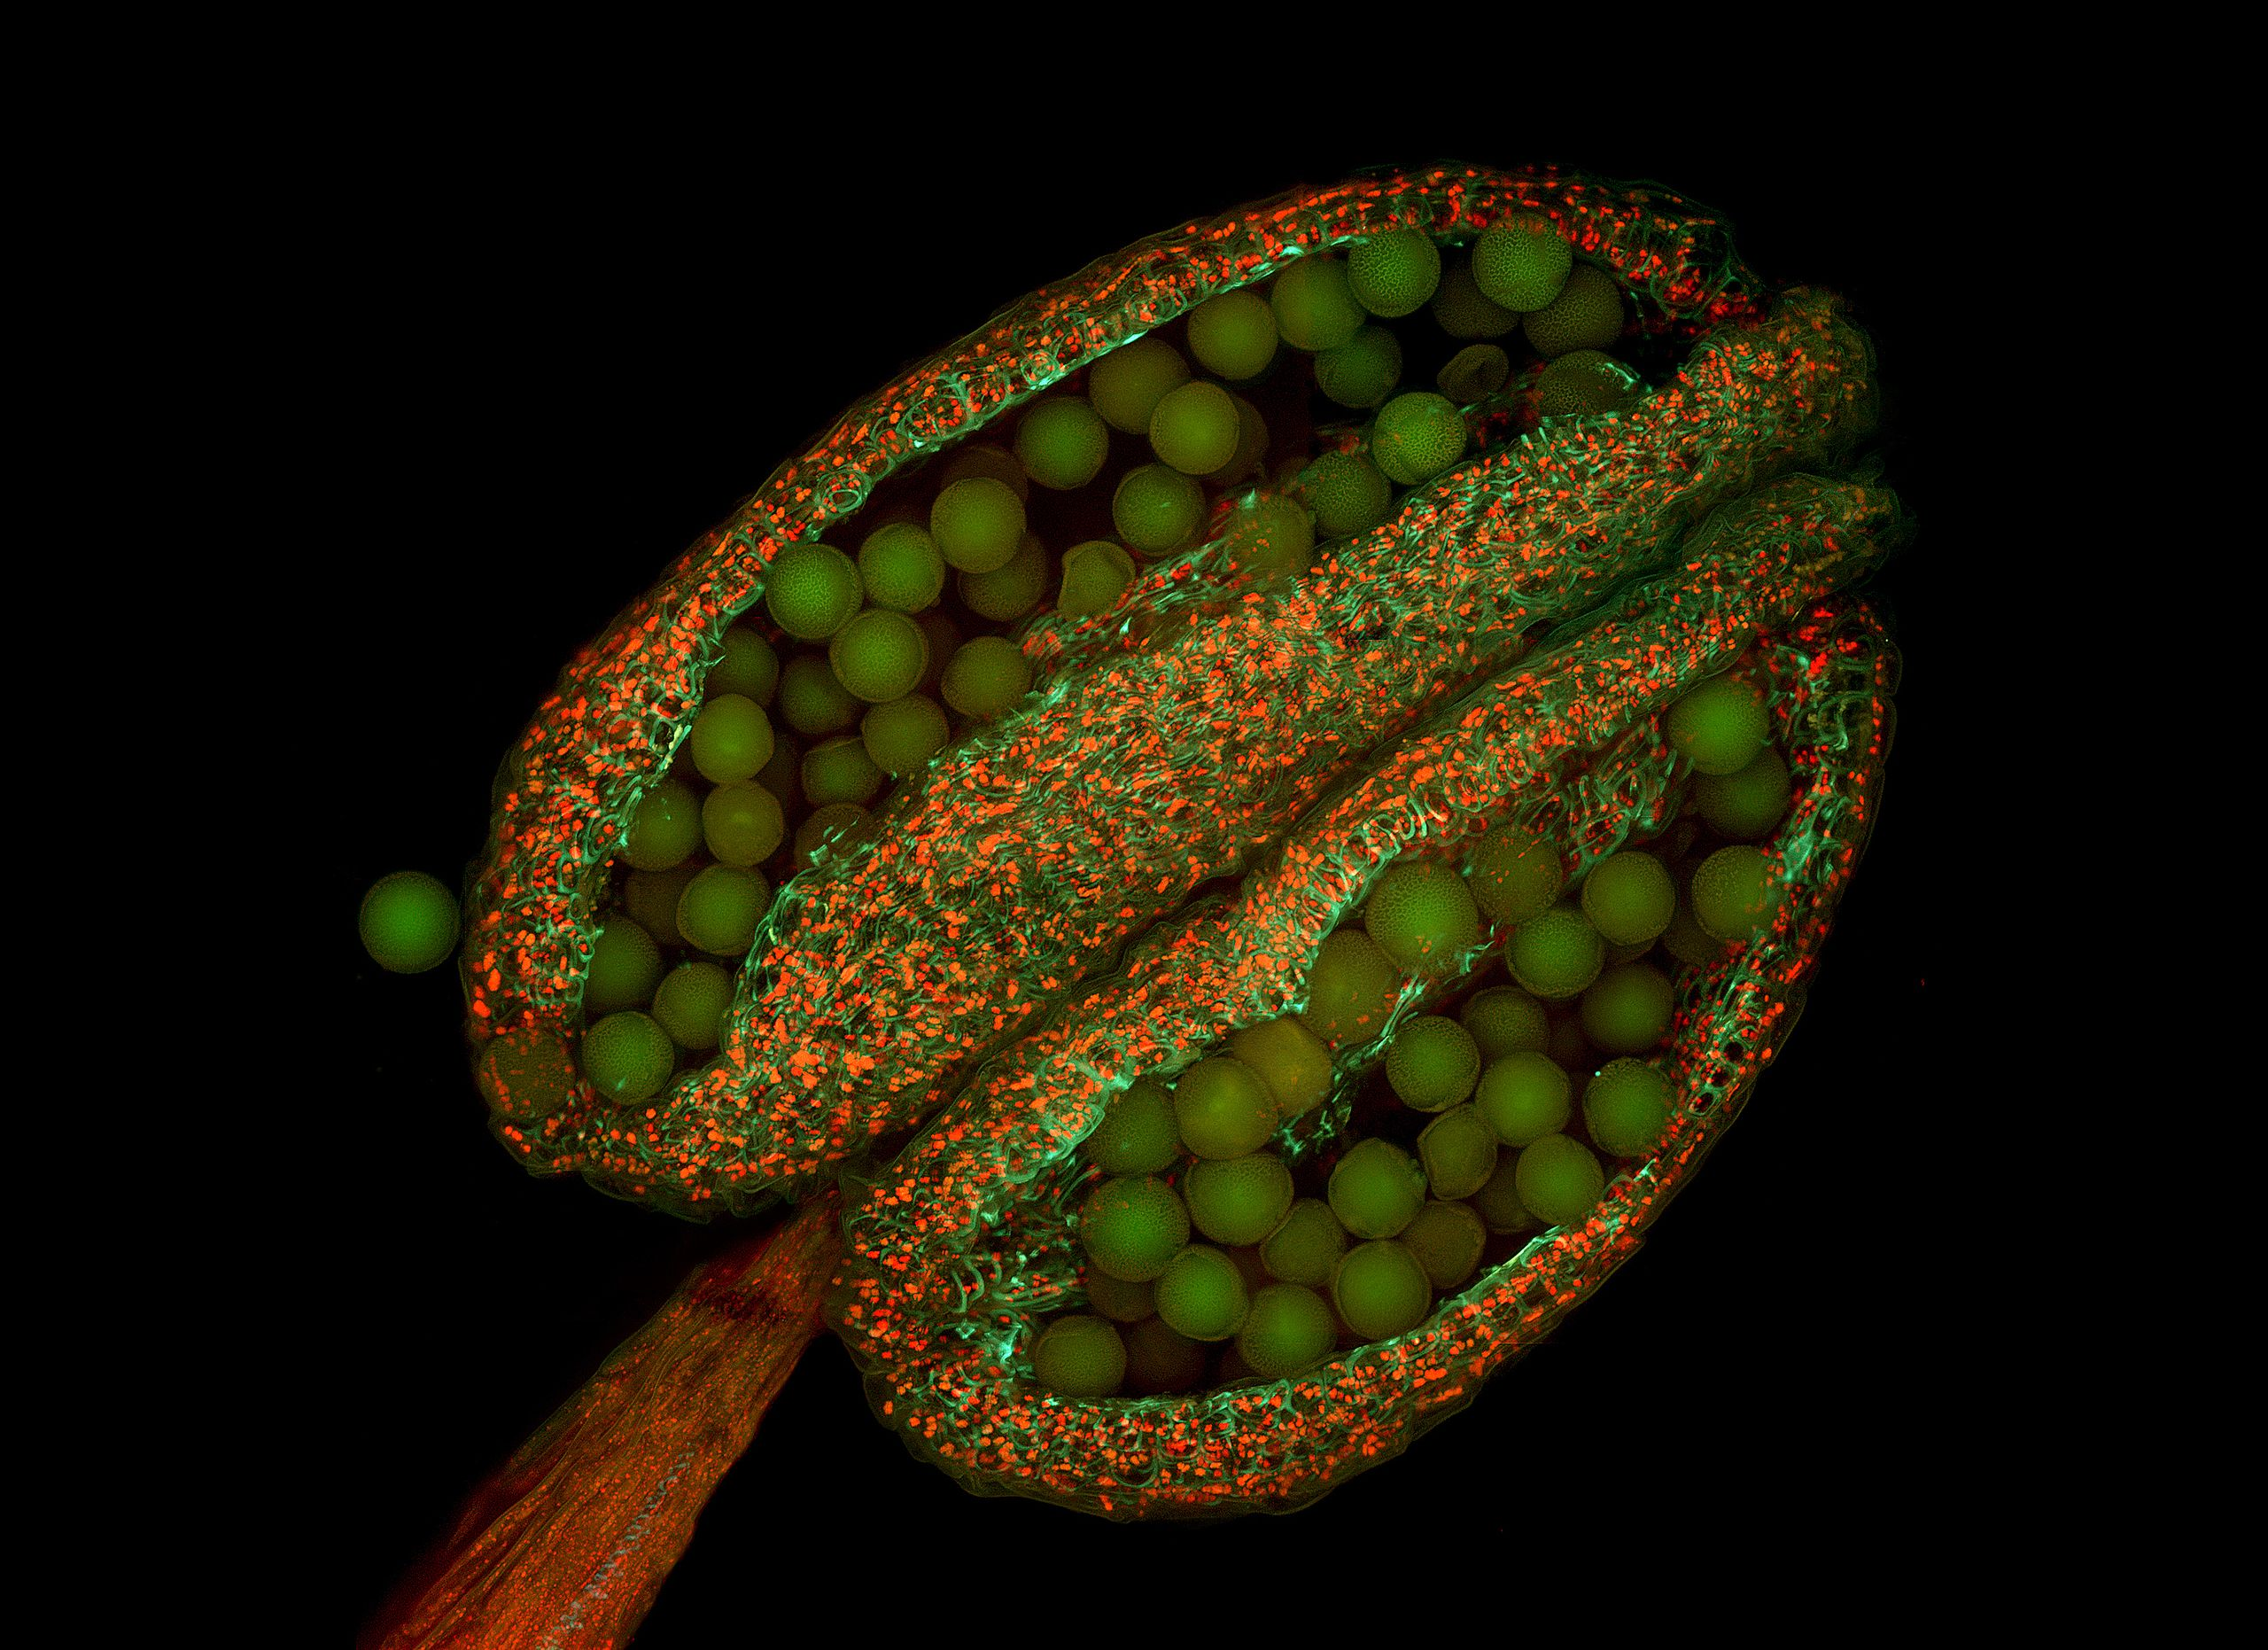
\includegraphics[width=\linewidth]{Tolmukapea.jpg}
% 	\caption{Anther of thale cress (Arabidopsis thaliana), fluorescence micrograph. Source: Heiti Paves, \href{https://commons.wikimedia.org/wiki/File:Tolmukapea.jpg}{https://commons.wiki-\\media.org/wiki/File:Tolmukapea.jpg}.}
% 	\label{fig:tcanther}
% \end{figure}

% Referencing a figure using its label: Figure \ref{fig:tcanther}.

% Aenean porttitor eros non pharetra congue. Proin in odio in dolor luctus auctor ac et mi. Etiam euismod mi sed lectus fringilla pretium. Phasellus tristique maximus lectus et sodales. Mauris feugiat ligula quis semper luctus. Nam sit amet felis sed leo fermentum aliquet. Mauris arcu dui, posuere id sem eget, cursus pulvinar mi. Donec nec lacus non lectus fermentum scelerisque et at nibh. Sed tristique, metus ac vestibulum porta, tortor lectus placerat lorem, et convallis tellus dolor eget ante. Pellentesque dui ligula, hendrerit a purus et, volutpat tempor lectus. Mauris nec purus nec mauris rhoncus pellentesque. Quisque quis diam sed est lacinia congue. Donec magna est, hendrerit sed metus vel, accumsan rutrum nibh.

% \begin{figure*} % Two column figure (notice the starred environment)
% 	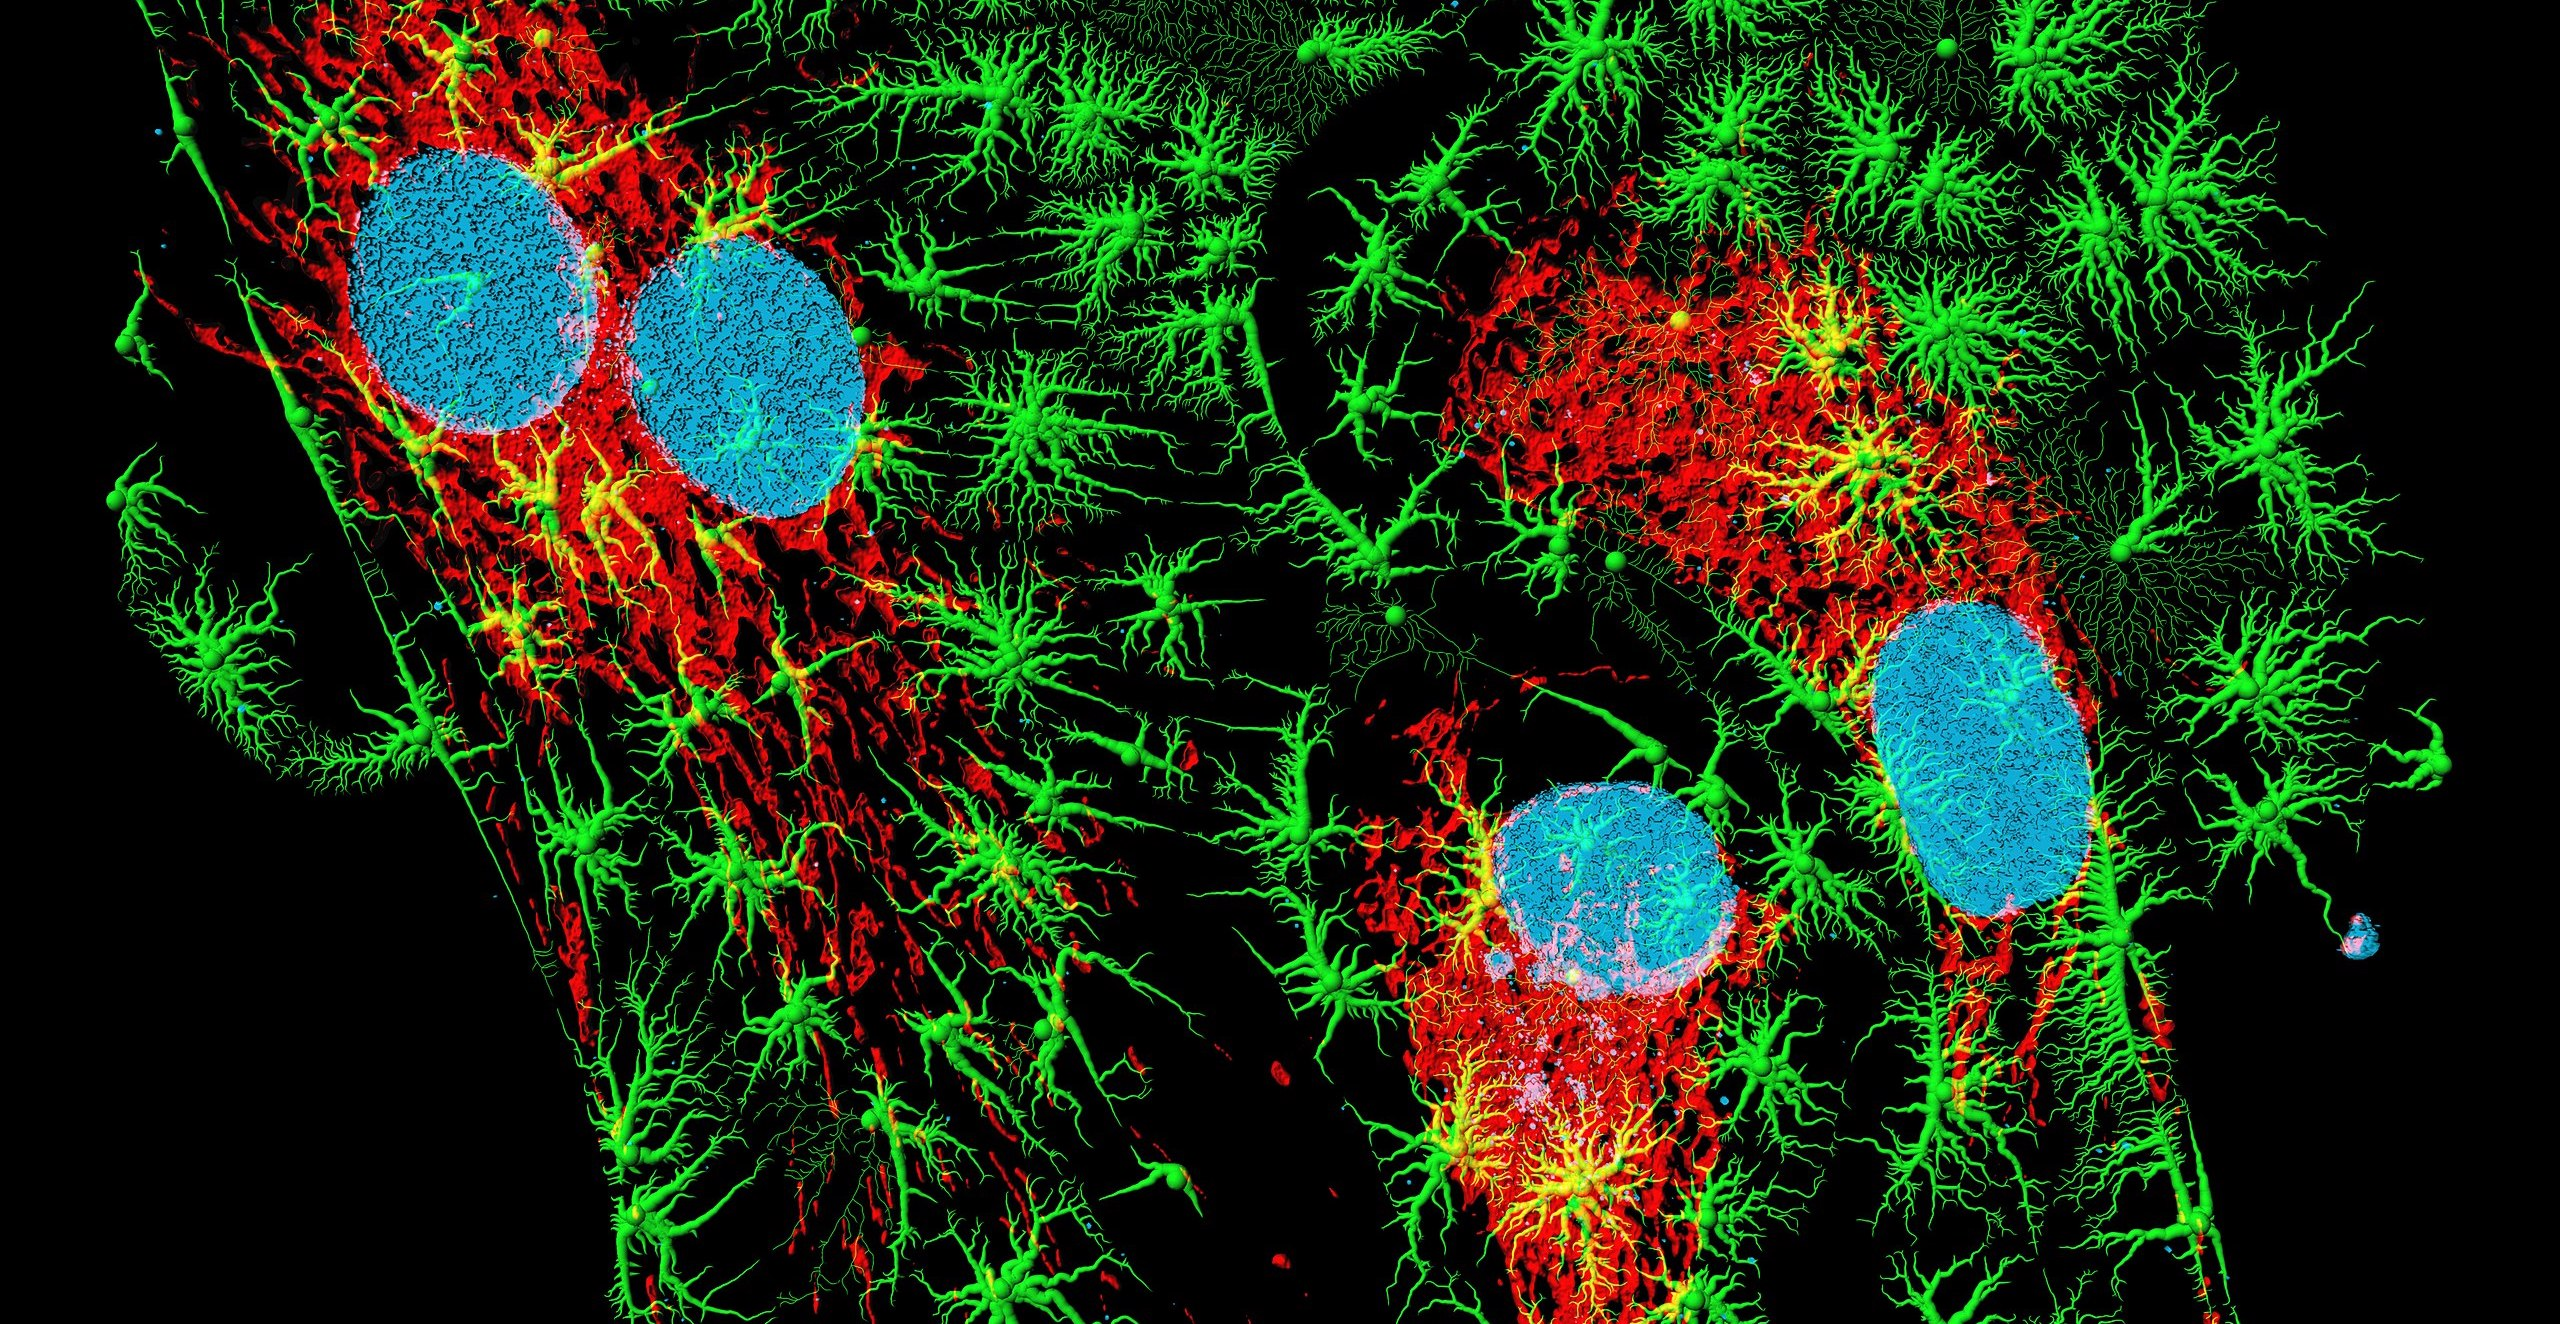
\includegraphics[width=\linewidth]{Fibroblastid.jpg}
% 	\caption{Bovine pulmonary artery endothelial cells in culture. Blue: nuclei; red: mitochondria; green: microfilaments. Computer generated image from a 3D model based on a confocal laser scanning microscopy using fluorescent marker dyes. Source: Heiti Paves, \href{https://commons.wikimedia.org/wiki/File:Fibroblastid.jpg}{https://commons.wikimedia.org/wiki/File:Fibroblastid.jpg}.}
% 	\label{fig:bpartery}
% \end{figure*}

% Orci varius natoque penatibus et magnis dis parturient montes, nascetur ridiculus mus. Etiam cursus lectus purus, tempus iaculis quam dictum tristique. Nam interdum sapien nec tempor mattis. Quisque id sapien nisi. Mauris vehicula ornare eros vel efficitur. Nulla consectetur, turpis quis fringilla tincidunt, mi neque iaculis lectus, vel commodo elit odio non ex. Duis facilisis, purus ac viverra iaculis, turpis lectus ultrices ante, ac vestibulum ligula magna in libero. Etiam tristique maximus lacinia. Vestibulum hendrerit, lacus malesuada laoreet blandit, sapien velit sollicitudin nunc, eu porttitor urna ligula at lorem. Aliquam faucibus eros in fermentum venenatis. Fusce consectetur congue pellentesque. Suspendisse at nisi sit amet est porttitor cursus. Cras placerat faucibus nunc, a laoreet justo dignissim sit amet.

% \subsection{International Support}

% \noindent àáâäãåèéêëìíîïòóôöõøùúûüÿýñçčšž

% \noindent ÀÁÂÄÃÅÈÉÊËÌÍÎÏÒÓÔÖÕØÙÚÛÜŸÝÑ

% \noindent ßÇŒÆČŠŽ

% \subsection{Links}

% This is a clickable URL link: \href{https://www.latextemplates.com}{LaTeX Templates}. This is a clickable email link: \href{mailto:vel@latextemplates.com}{vel@latextemplates.com}. This is a clickable monospaced URL link: \url{https://www.LaTeXTemplates.com}.

% %------------------------------------------------

% \section{Discussion}

% This statement requires citation \autocite{Richard:2005}. This statement requires multiple citations \autocite{Richard:2005,Richard:2005}. This statement contains an in-text citation, for directly referring to a citation like so: \textcite{Richard:2005}.

%----------------------------------------------------------------------------------------
%	 REFERENCES
%----------------------------------------------------------------------------------------

\printbibliography % Output the bibliography

%----------------------------------------------------------------------------------------

\appendix
\renewcommand{\thesection}{Appendix \Alph{section}:}
\renewcommand{\thesubsection}{\Alph{section}.\arabic{subsection}}
\onecolumn
\setlength{\parindent}{1em}
\setlength{\parskip}{1em}

\section{Supplementary Materials}
\label{sec:supplementary}

\subsection{Project Repository}
\label{sec:code}

\subsubsection{Project} \url{https://github.com/piranha-plants-as-charade}.
\subsubsection{Engine (Main Pipeline)} \url{https://github.com/piranha-plants-as-charade/engine}.
\subsubsection{Sample Inputs and Outputs} \url{https://github.com/piranha-plants-as-charade/results}.

\clearpage
\subsection{Transcription of the Melody Extraction Outputs for the Same Melody With Various Timbres}
\label{sec:sheet_music_melody}

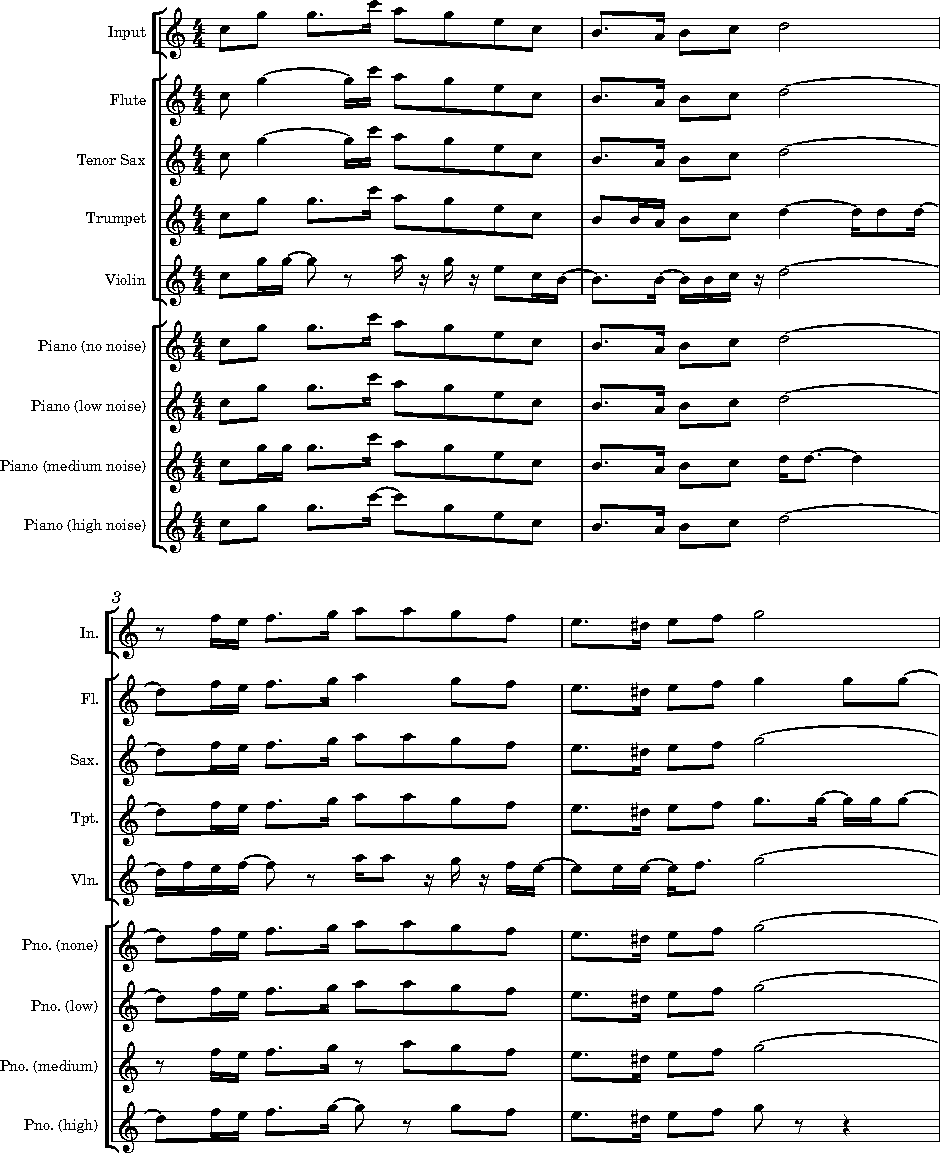
\includegraphics[page=1, width=\linewidth]{materials/piranha_melody.pdf}
\clearpage

\includegraphics[page=2, width=\linewidth]{materials/piranha_melody.pdf}
\clearpage

\clearpage
\subsection{Transcription of the Original and Generated Chord Progression for an Excerpt From ``Piranha Plants on Parade''}
\label{sec:sheet_music_melody}

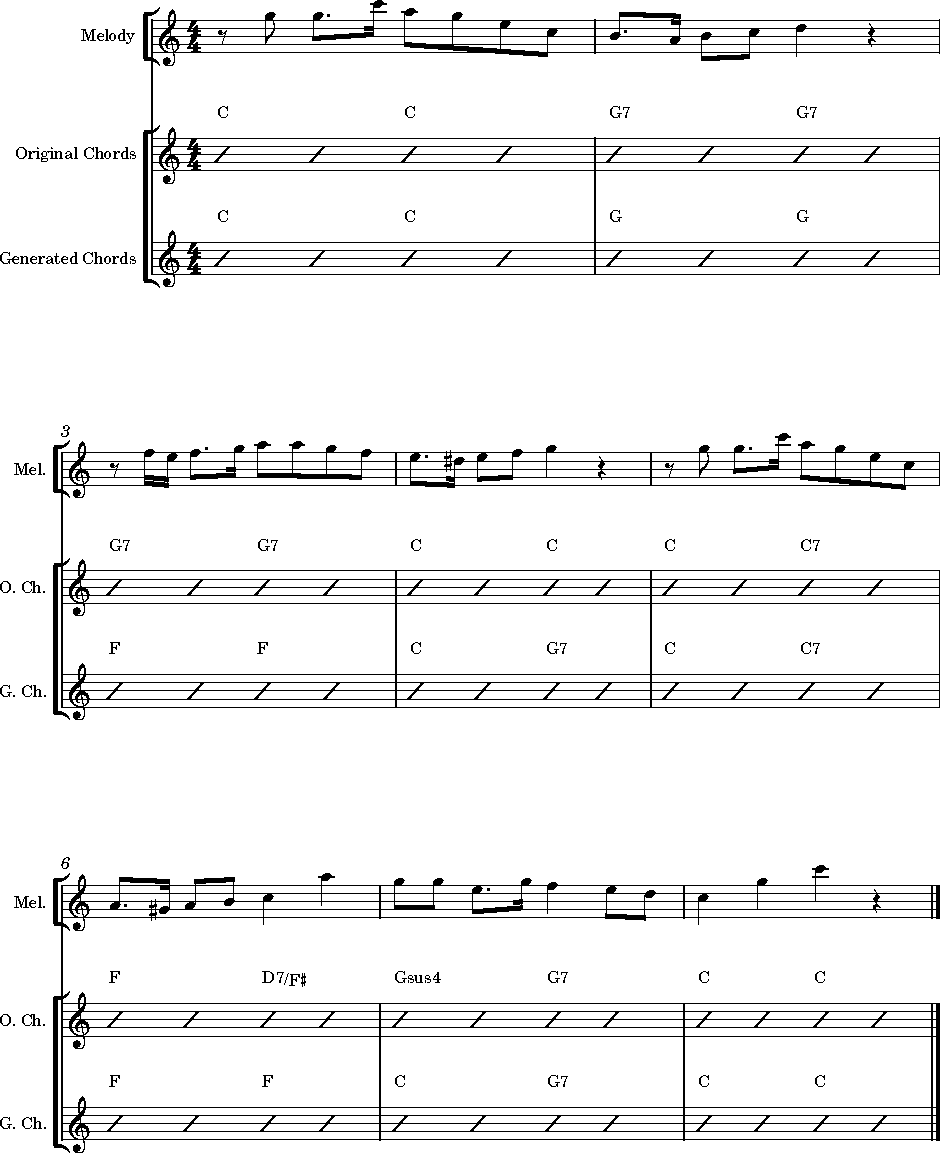
\includegraphics[page=1, width=\linewidth]{materials/piranha_chords.pdf}
\clearpage

% \includegraphics[page=2, width=\linewidth]{materials/piranha_melody.pdf}
% \clearpage

% \clearpage
% \subsection{Transcription of Generated ``Piranha Plants as Parade''}
% \label{sec:sheet_music_generated}

% 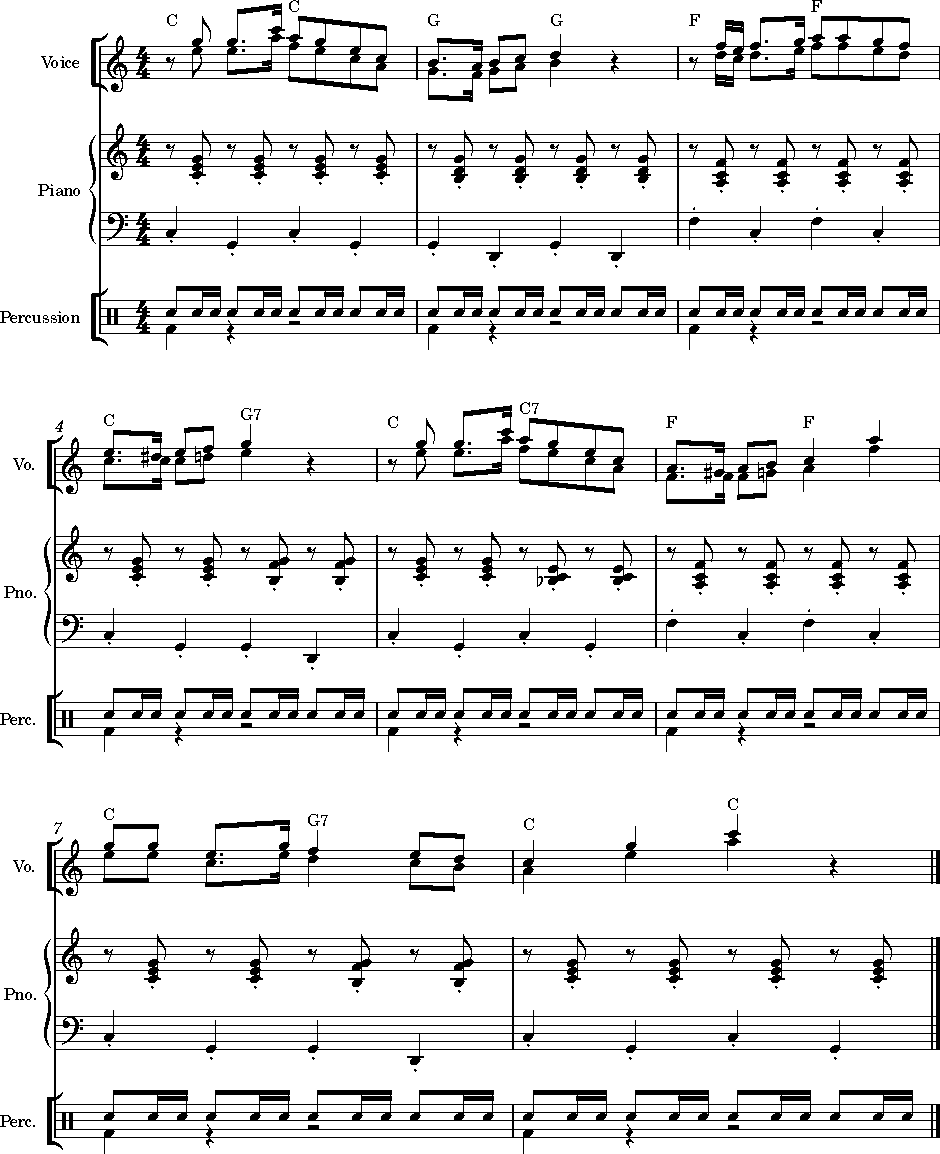
\includegraphics[page=1, width=\linewidth]{materials/piranha_generated.pdf}
% \clearpage

% \clearpage
% \subsection{Transcription of Original ``Piranha Plants on Parade''}
% \label{sec:sheet_music_original}

% This transcription is a simplification of ``Piranha Plants on Parade''. It has been transposed to the key of C Major to simplify comparisons with the outputs from Piranha Plants as Charade.

% 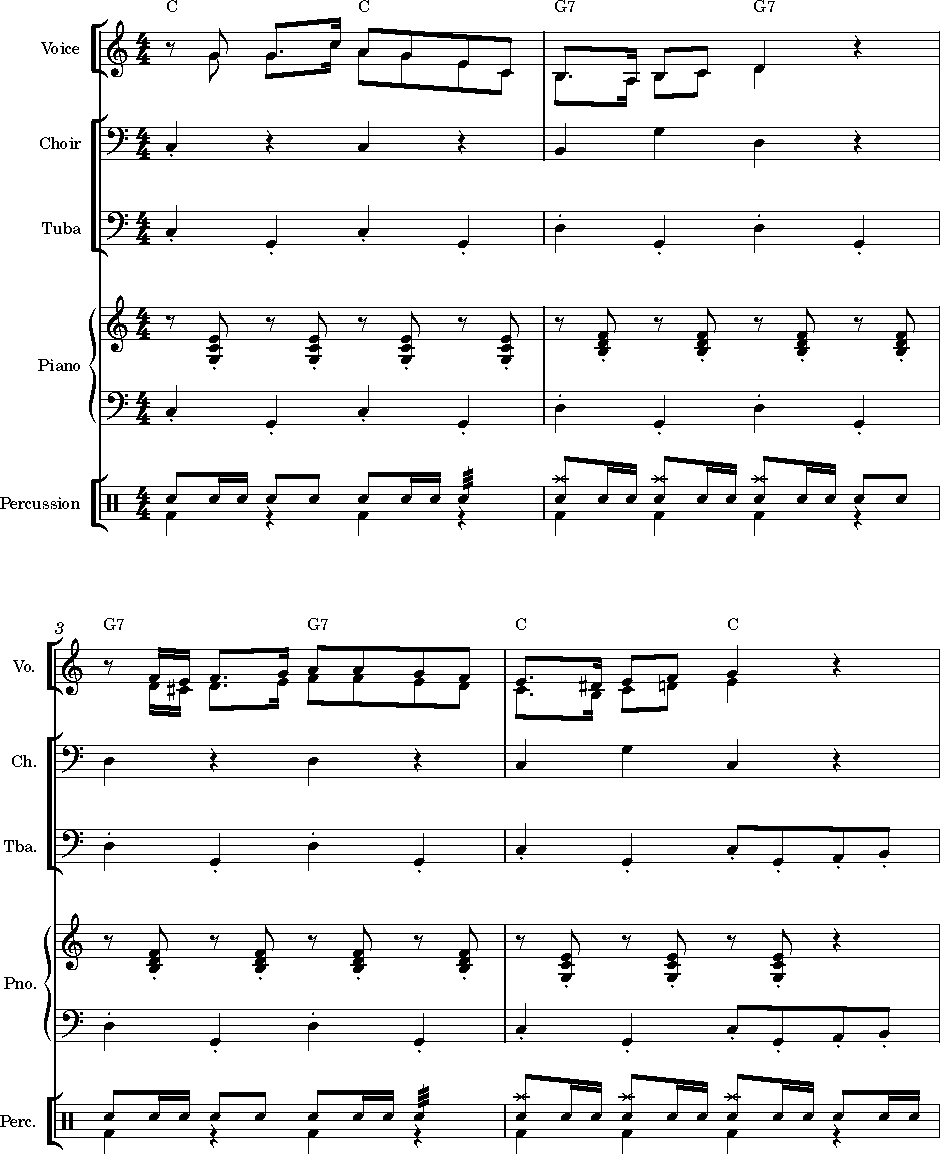
\includegraphics[page=1, width=\linewidth]{materials/piranha_original.pdf}
% \clearpage

% \includegraphics[page=2, width=\linewidth]{materials/piranha_original.pdf}
% \clearpage

\end{document}
